\documentclass{article}
\usepackage{amssymb, amsmath, amsthm}
\usepackage[margin=1in]{geometry}
\usepackage{verbatim}
\usepackage{graphicx}
\usepackage{hyperref} % \url \href
\usepackage{docmute}

\newtheorem{definition}{Definition}
\newtheorem{theorem}{Theorem}
\newcommand{\heff}{\mathbb{H}^{\text{eff}}}
\newcommand{\pfrac}[2]{\frac{\partial #1}{\partial #2}}

\begin{document}

\section{Two-orbital solution}
We illustrate the application of the direct solution method using the two (atomic) orbital problem. Suppose the 
value of the parameters $H_{11} = \varepsilon_1^0$, $H_{22} = \varepsilon_2^0$, $H_{12}$ are known, as well as 
for the overlap: $S_{11} = S_{22} = 1$ and $S_{12}$. 
\begin{align}
    (\varepsilon_1^0 - \varepsilon_1) c_{11} + (H_{12} - \varepsilon_1 S_{12}) c_{21} &= 0 \\
    (H_{12} - \varepsilon_2 S_{12}) c_{12} + (\varepsilon_2^0 - \varepsilon_2) c_{22} &= 0 \\ 
    S_{ii} = c_{1i}^2 + c_{2i}^2 + 2 c_{1i} c_{2i} S_{12} &= 1
\end{align}
the energies can be solved by the determinant:
\begin{align}
    \left| \begin{matrix}
        \varepsilon_1^0 - \varepsilon_i & H_{12} - \varepsilon_i S_{12} \\
        H_{12} - \varepsilon_i S_{12} & \varepsilon_2^0 - \varepsilon_i
    \end{matrix} \right| &= 0 
\end{align}
therefore given by a second order equation:
\begin{equation}
    (\varepsilon_1^0 - \varepsilon_i)(\varepsilon_2^0 - \varepsilon_i) - (H_{12} - \varepsilon_i S_{12})^2 = 0
\end{equation}

\subsection{Degenerate case}
When $\varepsilon_1^0 = \varepsilon_2^0 = \varepsilon^0$, the solution for the energy can be found to be:
\begin{align}
    \varepsilon_1 = \frac{\varepsilon^0 + H_{12}}{1 + S_{12}} \approx \varepsilon^0 + (H_{12} - \varepsilon^0 S_{12}) - S_{12} (H_{12} - \varepsilon_i^0 S_{12}) \\
    \varepsilon_2 = \frac{\varepsilon^0 - H_{12}}{1 - S_{12}} \approx \varepsilon^0 - (H_{12} - \varepsilon^0 S_{12}) - S_{12} (H_{12} - \varepsilon_i^0 S_{12}) 
\end{align}
$S_{12} > 0$ and $H_{12} < 0$, we have thus $H_{12} - \varepsilon^0 S_{12} < 0$ so that $\varepsilon_1 < \varepsilon_2$, which are further shifted down by a small amount 
given by the second term.
The normalization coefficient can be solved using the secular relationship. We have:
\begin{equation}
    \frac{c_{21}}{c_{11}} = 1; \quad \frac{c_{22}}{c_{12}} = -1
\end{equation}
and the wave functios are:
\begin{align}
    \psi_1 = \frac{1}{\sqrt{2 + 2 S_{12}}} (\chi_1 + \chi_2) \\
    \psi_2 = \frac{1}{\sqrt{2 - 2 S_{12}}} (\chi_1 - \chi_2)
\end{align}

\subsection{Nondegenerate case}
Approximate results can be given for non-degenerate cases, with the solution for energies:
\begin{align}
    \varepsilon_1 \approx \varepsilon_1^0 + \frac{(H_{12} - \varepsilon_1^0 S_{12})^2}{\varepsilon_1^0 - \varepsilon_2^0} < \varepsilon_1^0 \\
    \varepsilon_2 \approx \varepsilon_2^0 + \frac{(H_{12} - \varepsilon_1^0 S_{12})^2}{\varepsilon_2^0 - \varepsilon_1^0} > \varepsilon_2^0
\end{align}
since we take $\varepsilon_2^0 > \varepsilon_1^0$. Furthermore, we have:
\begin{equation}
    \varepsilon_2^0 - \varepsilon_2 < \varepsilon_1 - \varepsilon_1^0
\end{equation}
The solution for the coefficients are given for $\psi_1$:
\begin{gather}
    \psi_1 \approx \left(1 - tS_{12} - \frac{1}{2}t^2\right) \chi_1 + t \chi_2 \\
    t = \frac{H_{12}-\varepsilon_1^0S_{12}}{\varepsilon_1^0 - \varepsilon_2^0} > 0
\end{gather}
so that $\psi_1$ is obtained by combining $\chi_1$ and $\chi_2$ in phase. 
The solution for $\psi_2$ is:
\begin{gather}
    \psi_2 \approx t' \chi_1 + \left( 1 - t' S_{12} - \frac{1}{2}t'^2 \right) \chi_2 \\
    t' = \frac{H_{12}-\varepsilon_2^0S_{12}}{\varepsilon_2^0 - \varepsilon_1^0} < 0
\end{gather}
$\psi_2$ is obtained by mixing $\chi_1$ out of phase with $\chi_2$. 

\subsection{Charge Transfer Interaction}
In the above non-degenerate case, if we initially have two electrons on 
the lower energy orbitals and we turn on the interaction so that the bonding 
and antibonding orbitals are formed, such as shown in figure \ref{F:charge_transfer}. 
It can be seen that the net effect of forming the bond is the transfer of charge 
from the left atomic orbitals to the right, as given by the perturbed wavefunction:
\begin{equation*}
    \psi_1 \approx (1-t) \chi_1 + t \chi_2
\end{equation*}
Initutively, we can understand such charge transfer as follows: although the 
state on the right has a higher energies than that on the left, the area between 
the two ions, especially near the left one, become more electronegative and attract 
electrons to this region. The total effect is therefore a slight reduction in 
energy. This type of bonding situation is called \emph{charge transfer interaction}.
\begin{figure}[h!]
    \centering
    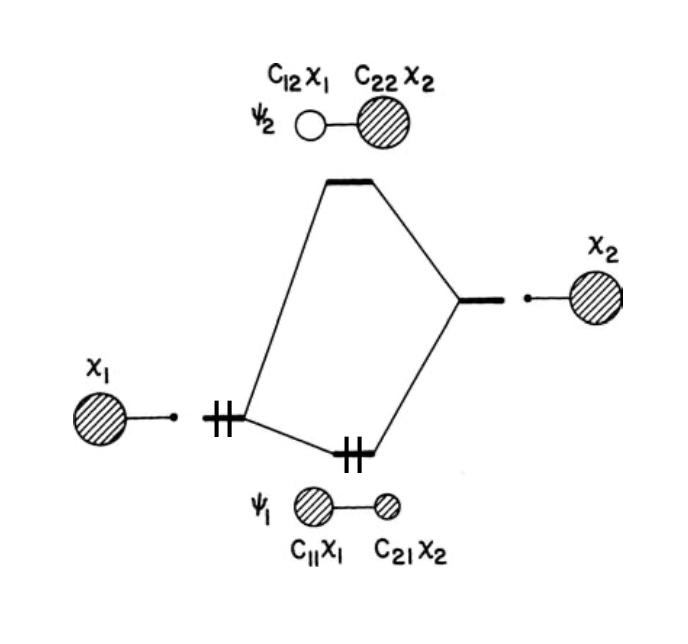
\includegraphics[width=3in]{F_charge_transfer.png}
    \caption{Orbital diagram in the case of charge transfer interaction}
    \label{F:charge_transfer}
\end{figure}



\end{document}
